\documentclass[11pt]{article}
\usepackage[english]{babel}
\usepackage[utf8]{inputenc}
\usepackage{ifthen}
\selectlanguage{english}
\usepackage[pdftex]{graphicx}
\usepackage{fancyhdr}
\usepackage{subfigure}
\usepackage[hmargin=1in,vmargin=1in]{geometry}
\usepackage{setspace}
\usepackage{url}
%\usepackage{fancyhdr}
%\pagestyle{fancy}
%%% ----------------------------------------------------------------------

%\rfoot{\thepage}
%\cfoot{}
%\lhead{}
\pagestyle{fancy}
\lhead{GSBGEN 390 : Individual Research \\ Sponsoring Professor William Barnett}
\rhead{Pedro Alves Ribeiro Côrte-Real \\ SUID: 005575591}
\lfoot{}
\rfoot{}
\setlength{\headheight}{30pt}

\title{Final Writeup}
\date{}
\author{}

\begin{document}

\maketitle
\thispagestyle{fancy}

\section{Introduction}

Previous work on building quantitative measures based on the source are either outdated\cite{sloccount} or target only a specific project\cite{lwnstats,gnomecensus}.

\section{Methodology}

\section{Preliminary Results}

\begin{figure}[htb]
  \begin{center}
    \subfigure[Churn vs Size]{\label{churn:size}\includegraphics[width=80mm]{../generated/sizevschurn/sizevschurn.pdf}}
    \subfigure[Churn per section]{\label{churn:section}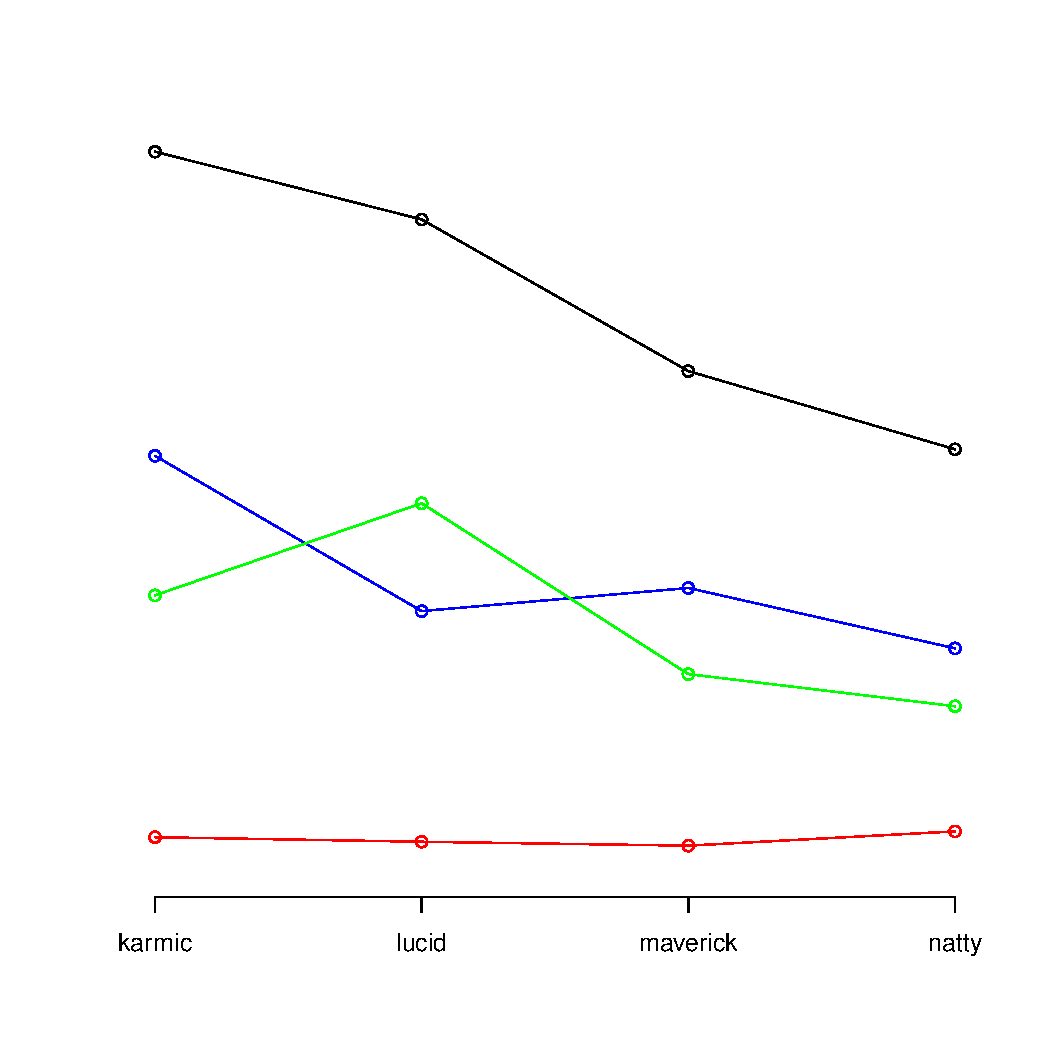
\includegraphics[width=80mm]{../generated/sectionsplit/sectionsplit.pdf}}
  \end{center}
  \caption{Package to package churn in the last four Ubuntu releases}
  \label{fig:churn}
\end{figure}

\begin{figure}[htb]
  \begin{center}
    \subfigure[Total]{\label{gnuinlinux:total}\includegraphics[height=60mm]{../generated/gnuinlinux/totalsplit.pdf}}
    \subfigure[GNU software]{\label{gnuinlinux:gnu}\includegraphics[height=60mm]{../generated/gnuinlinux/gnusplit.pdf}}
  \end{center}
  \caption{LOC split of projects in Ubuntu natty's main repository}
  \label{fig:gnuinlinux}
\end{figure}

\section{Future Work}

Of the existing work:

- Accumulate enough popcon timeseries data to do a meaningful comparison
- Create the maturity variable based on the bug reports
- Small technical fixes in the way churn and LOC are calculated

Of future other sources of work:

- Do comparisons based on Fedora for a different view over the same available component pieces
- Repurpose the same code for Debian and see if the Canonical effect can be detected in statistically significant ways
- Start looking at finer grained data from git/mercurial that allows per-line blame and other such goodies
- Explore github and its dynamics as a social graph on top of a code repository

\section{Conclusion}

\newpage
\begin{thebibliography}{9}

\bibitem{sloccount}
David A. Wheeler,
\emph{More Than a Gigabuck: Estimating GNU/Linux's Size}\\
\url{http://www.dwheeler.com/sloc/redhat71-v1/redhat71sloc.html}\\
June 30, 2001 (updated July 29, 2002)

\bibitem{lwnstats}
Jonathan Corbet,
\emph{2.6.39 development statistics}\\
\url{https://lwn.net/Articles/442229/}\\
May 10, 2011

\bibitem{gnomecensus}
Neary Consulting,
\emph{The GNOME Census: Who writes GNOME?}\\
\url{http://www.neary-consulting.com/docs/GNOME_Census.pdf}\\
July 28, 2010


\bibitem{ubuntureleases}
\emph{List of Ubuntu releases}\\
\url{https://wiki.ubuntu.com/Releases}

\bibitem{prelimresults}
Pedro Côrte-Real,
\emph{Preliminary Results from Open Source Evolution Analysis}\\
\url{http://pedrocr.net/text/preliminary-results-open-source-evolution}\\
May 12 2011

\bibitem{gnuinlinux}
Pedro Côrte-Real,
\emph{How much GNU is there in GNU/Linux?}\\
\url{http://pedrocr.net/text/how-much-gnu-in-gnu-linux}\\
May 31 2011

\bibitem{repo}
\emph{Source repository}\\
\url{https://github.com/pedrocr/codecomp}

\end{thebibliography}

\end{document}
